\documentclass[portrait,final,a1paper,fontscale=0.3]{baposter}

\usepackage{calc}
\usepackage{graphicx}
\usepackage{amsmath}
\usepackage{amssymb}
\usepackage{relsize}
\usepackage{multirow}
\usepackage{rotating}
\usepackage{bm}
\usepackage{url}

\usepackage{graphicx}
\usepackage{multicol}
\usepackage{amsthm}
\usepackage{amssymb}
\usepackage{mathtools}
\DeclarePairedDelimiter\abs{\lvert}{\rvert}
\DeclarePairedDelimiter\norm{\lVert}{\rVert}
\DeclarePairedDelimiter\inner{\langle}{\rangle}
\def\P{\mathcal{P}}
\DeclareMathOperator*{\argmin}{argmin}
\theoremstyle{definition}
\newtheorem{definition}{Definition}
\newtheorem{proposition}{Proposition}
\newtheorem{example}{Example}
\newtheorem{lemma}{Lemma}
\newtheorem{corollary}{Corollary}
\newtheorem{theorem}{Theorem}
\usepackage{algorithm}
\usepackage{algorithmic}
\makeatletter
\newcommand{\algorithmicfunction}{\textbf{function}}
\newcommand{\algorithmicendfunction}{\algorithmicend\ \algorithmicfunction}
\newenvironment{ALC@func}{\begin{ALC@g}}{\end{ALC@g}}
\newcommand{\FUNCTION}[2][default]{\ALC@it\algorithmicfunction\ #2\ %
\textbf{:}%
\ALC@com{#1}\begin{ALC@func}}
\ifthenelse{\boolean{ALC@noend}}{
    \newcommand{\ENDFUNCTION}{\end{ALC@func}}
  }{
    \newcommand{\ENDFUNCTION}{\end{ALC@func}\ALC@it\algorithmicendfunction}
  }
\makeatother

\usepackage{palatino}

\newcommand{\captionfont}{\footnotesize}


\setlength{\columnsep}{1.5em}
\setlength{\columnseprule}{0mm}

\newcommand{\compresslist}{%
\setlength{\itemsep}{1pt}%
\setlength{\parskip}{0pt}%
\setlength{\parsep}{0pt}%
}


\begin{document}


\definecolor{stevensred}{HTML}{82318E}
\definecolor{stevensgray}{rgb}{0.60392, 0.596, 0.60392}

\begin{poster}%
  {
  grid=false,
  colspacing=1em,
  bgColorOne=white,
  bgColorTwo=white,
  borderColor=stevensgray,
  headerColorOne=stevensred,
  headerColorTwo=stevensred,
  headerFontColor=white,
  boxColorOne=white,
  boxColorTwo=stevensgray,
  textborder=rectangle,
  eyecatcher=true,
  headerborder=closed,
  headerheight=0.13\textheight,
  headershape=rectangle,
  headershade=shadelr,
  headerfont=\Large\bf\textsc, %Sans Serif
  textfont={\setlength{\parindent}{1.5em}},
  boxshade=plain,
  background=plain,
  linewidth=2pt
  }
  {
  		
\includegraphics[height=9.0em]{thu.jpg}
  } % Empty space, replace with image if desired
  {\bf \textsc{ Info-Detection: An Information-Theoretic Approach to Detect Outlier } }
  {\textsc{  Feng Zhao, Fei Ma, Yang Li, Shao-Lun Huang and Lin Zhang \\ Tsinghua-Berkeley Shenzhen Institute, Tsinghua University}}
  {% The makebox allows the title to flow into the logo, this is a hack because of the L shaped logo.
  }

    \newcommand{\colouredcircle}{%
      \tikz{\useasboundingbox (-0.2em,-0.32em) rectangle(0.2em,0.32em); \draw[draw=black,fill=lightblue,line width=0.03em] (0,0) circle(0.18em);}}

  \headerbox{Introduction}{name=problem,column=0,row=0}{

Outlier detection is one of major task in unsupervised learning. We propose a cluster analysis based method called Info-Detection. It can determine the number of outliers automatically. To implement Info-Detection, we use some graph theory techniques and make it usable on small dataset.

}

  \headerbox{References}{name=references,column=0,above=bottom}{
    \smaller
    \bibliographystyle{ieee}
    \renewcommand{\section}[2]{\vskip 0.05em}
      \begin{thebibliography}{1}\itemsep=-0.01em
      \setlength{\baselineskip}{0.4em}
      
\bibitem{sparsekernel} C.~Chan, A.~Al-Bashabsheh, Q.~Zhou, T.~Kaced, and T.~Liu.
\newblock Info-clustering: A mathematical theory for data clustering.
\newblock {\em IEEE Transactions on Molecular, Biological and Multi-Scale
  Communications}, 2(1):64--91, 2016.
  
\bibitem{RN4}
Vladimir Kolmogorov.
\newblock A faster algorithm for computing the principal sequence of partitions
  of a graph.
\newblock {\em Algorithmica}, 56(4):394--412, 2010.

\bibitem{RN7}
Kiyohito Nagano, Yoshinobu Kawahara, and Satoru Iwata.
\newblock Minimum average cost clustering.
\newblock {\em Advances in Neural Information Processing
  Systems 23}, pages 1759--1767. Curran Associates, Inc., 2010.

      \end{thebibliography}
   \vspace{0.05em}
  }

  \headerbox{Info-clustering}{name=method,column=0,below=problem, above=references}{
Info-Detection derives from info-clustering.

Info-clustering is an information theoretic clustering method and
can produce hierachical tree for the random variables to be clustered. 

Info-Detection defines a multi-variate information for a directed graph
which can be used as clustering criterion.


\hspace{-1em}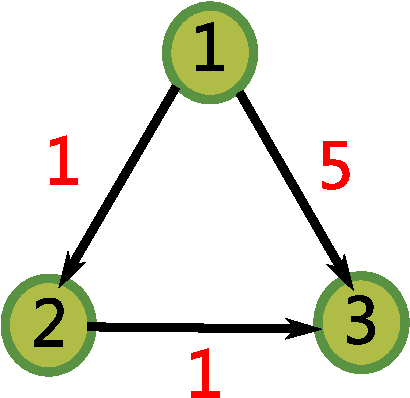
\includegraphics[width=\linewidth]{img/example_directed.pdf}


}

\headerbox{Formulation of Info-Detection}{name=formulation,column=1,span=2, row=0}{

Info-clustering has a series of threshold values and we use the largest one to distinguish inliers from outliers.

To make predictions on new observation, theoretically we can re-compute for the whole graph. We have shown that this is equivalent to use a simple similarity summation scheme:
\begin{equation*}
 \sum_{i \textrm{ is inliner} } w_{ij} 	 \mathop{\gtreqless}_{j \textrm{ is outlier}}^{j \textrm{ is inliner}} \textrm{ threshold }
\end{equation*}

\hspace{-1.2em}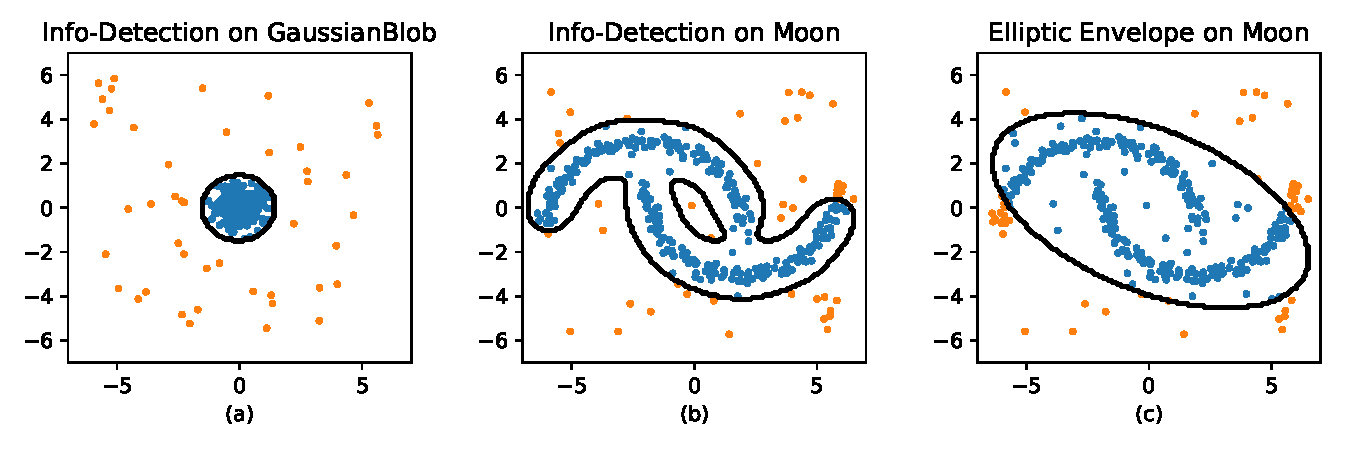
\includegraphics[width=\linewidth]{img/outlier_boundary_illustration}

}

\headerbox{Algorithm}{name=algorithm,column=1,span=2, below=formulation}{



Info-Detection criterion derives from the hierarchical tree of info-clustering. This tree is related with a special
structure in graph theory called principal sequence of partition.

We make use of the property of hierarchical structure and propose an improved algorithm to compute this structure. This decreases the time complexity from $O(n^5)$ to $O(n^4)$ for dense graphs in general.

{
\hspace{-1em}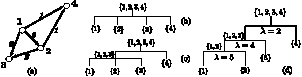
\includegraphics[width=\linewidth]{img/alg_illustration.pdf}
}

After the tree structure and critical values are obtained, we use the largest value as the detection threshold and the corresponding childrens as inliners.
}



  \headerbox{Experimental Results}{name=experiment,column=1, span=2,below=algorithm, above=bottom}{
\vspace{-0.3em}
\hspace{-1.2em}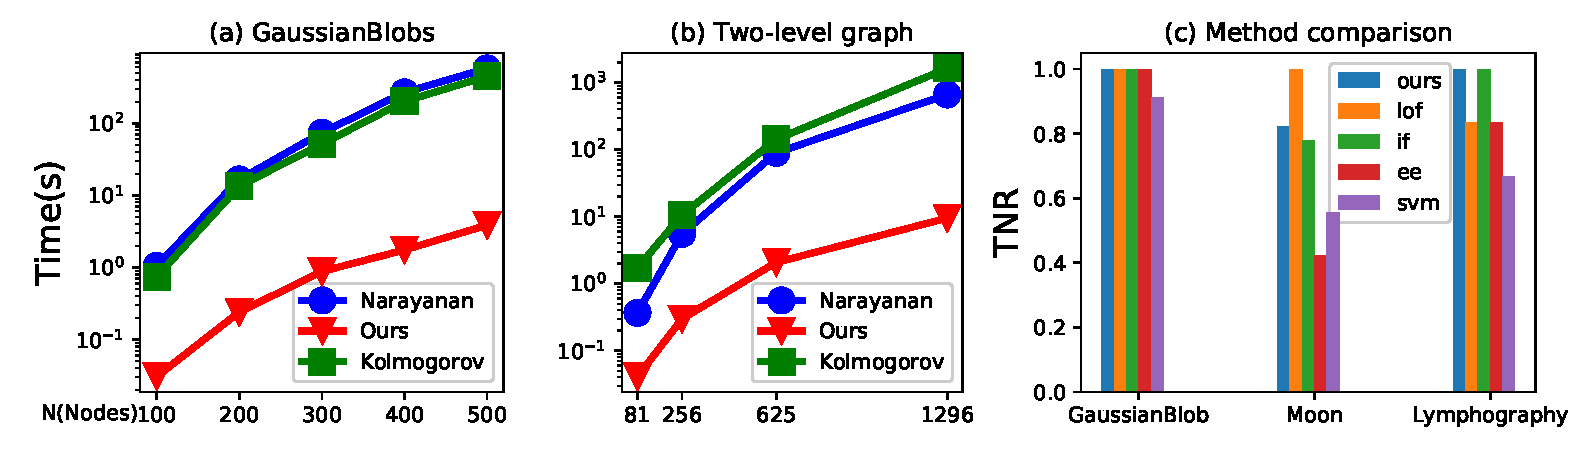
\includegraphics[width=\linewidth]{img/experimental_results}
}


\end{poster}

\end{document}

